%%%%%%%%%%%%%%%%%%%%%%
\documentclass{singlecol-new}
%%%%%%%%%%%%%%%%%%%%%%

\usepackage{natbib,stfloats}
\usepackage{mathrsfs}
\usepackage{natbib}
\usepackage{url}
\usepackage[pdftex]{graphicx}
\usepackage[utf8]{inputenc}
\usepackage{newunicodechar}
\usepackage[center]{caption}

\newcommand{\textprime}{\ensuremath{'}}
\newunicodechar{′}{\textprime}

\def\newblock{\hskip .11em plus .33em minus .07em}

\theoremstyle{TH}{
\newtheorem{lemma}{Lemma}
\newtheorem{theorem}[lemma]{Theorem}
\newtheorem{corrolary}[lemma]{Corrolary}
\newtheorem{conjecture}[lemma]{Conjecture}
\newtheorem{proposition}[lemma]{Proposition}
\newtheorem{claim}[lemma]{Claim}
\newtheorem{stheorem}[lemma]{Wrong Theorem}
\newtheorem{algorithm}{Algorithm}
}

\theoremstyle{THrm}{
\newtheorem{definition}{Definition}[section]
\newtheorem{question}{Question}[section]
\newtheorem{remark}{Remark}
\newtheorem{scheme}{Scheme}
}

\theoremstyle{THhit}{
\newtheorem{case}{Case}[section]
}

\makeatletter
\def\theequation{\arabic{equation}}




%\JOURNALNAME{\TEN{\it Int. J. System Control and Information
%Processing,
%Vol. \theVOL, No. \theISSUE, \thePUBYEAR\hfill\thepage}}%
%
%\def\BottomCatch{%
%\vskip -10pt
%\thispagestyle{empty}%
%\begin{table}[b]%
%\NINE\begin{tabular*}{\textwidth}{@{\extracolsep{\fill}}lcr@{}}%
%\\[-12pt]
%Copyright \copyright\ 2012 Inderscience Enterprises Ltd. & &%
%\end{tabular*}%
%\vskip -30pt%
%%%\vskip -35pt%
%\end{table}%
%}
\makeatother

%%%%%%%%%%%%%%%%%
\begin{document}%
%%%%%%%%%%%%%%%%%

\setcounter{page}{1}

%\LRH{K. Ho \& E. Koh}

\RRH{\renewcommand{\arraystretch}{0.8}\raisebox{4.2pt}[0pt]{\begin{tabular}{l}Metagenomic Analysis of Ruminal Microbiota Composition\\ Based on 16S rRNA Amplicon Sequences Using Qiime2 Pipeline\end{tabular}}}%

\VOL{1}

\ISSUE{1}

\PUBYEAR{2019}

\BottomCatch

\CLline

\subtitle{}

\title{Metagenomic Analysis of Ruminal Microbiota Composition Based on 16S rRNA Amplicon Sequences Using Qiime2 Pipeline}


%
%\authorA{Kiet Ho}
%
%\affA{Department of Computing Science,\\ Trinity Western University,\\ Langley, BC, Canada \\
%E-mail: kiet.kelvinh@gmail.com}
%
%
%\authorB{Eunhan Koh}
%\affB{Department of Biotechnology,\\ Trinity Western University,\\ Atlanta, BC, Canada \\
%E-mail: eunhankoh@gmail.com}
%

%
%
\begin{abstract}
% Abstract: approximately 100 words, maximum 150. 
The emergence of bioinformatic analysis pipelines in recent years have allowed researchers to generate insightful data regarding microbiomes in a cost-effective manner. QIIME (Quantitative Insights Into Microbial Ecology) is one of the bioinformatic analysis pipelines that is mentioned frequently in the science community. As the successor of QIIME, QIIME2 is expected to be an even more robust and sophisticated pipeline for analyzing microbiomes. Even though there are many suggested pipelines for QIIME2, each pipeline has different workflows and requirements that make using QIIME2 difficult for inexperienced users. In this study, a QIIME2 pipeline suitable for the analysis of ruminal microbiota will be constructed, using data provided by Lopez-Garcia et al.. This pipeline will enable users to become familiar with QIIME2, generate a taxonomic profile of ruminal microbiota, and create a phylogenetic tree.

\end{abstract}

\KEYWORD{Metagenomic analysis, Ruminal microbiome, 16S rRNA amplicon sequences, Bioinformatics pipeline, QIIME2, Taxonomy, Phylogeny.}


\maketitle


%%%%%%%%%%%%%%%%%%%%%%%%%%%%%%%%%%%%%%%%%%%%%%%%%%%%%%%%%%
 \section{Introduction}


Cellulose-rich feeds are digested with the help of rumen microbiota in cattle. By doing so, digested metabolites are used by the microbes themselves to proliferate and the host cattle use them as a source of nutrients. The symbiotic relationship evident here is critical for cattle's survival. Studying the composition of rumen microbiome is an interest posed by researchers around the world because it has many implications, such as its effect on climate change, animal production and the health of cattle \citep{mcgovern2018evaluating}.\linebreak

The field of microbiome analysis has improved immensely due to innovations in computing and sequencing technology. Researchers can determine the microbial diversity of a community by sequencing conserved regions of the microbial genome that can reveal information about their phylogeny \citep{de2017novel}. This conserved region that is most commonly sequenced in the science community is the 16S rRNA gene \citep{de2017novel, janda200716s}. Nowadays, the variable region 4 (V4) that is present in the 16S rRNA gene is amplified and sequenced most frequently, especially the 515 to 806 fragment. This is due to the general consensus in the science community that the indicated region will provide the most optimal classification \citep{de2017novel}.\linebreak

In order to know what type of microorganisms are present in a sample, researchers must assign taxonomy by analyzing the sequenced reads of the 16S rRNA gene. This is done with the help of bioinformatics analysis pipelines, which are ever-increasing in number \citep{siegwald2017assessment}. Recently, the bioinformatics tool QIIME has received positive feedback from active researchers on the topic of metagenomics analysis \citep{caporaso10}. By examining the DNA of microbes, researchers can determine the composition of microbes in a given community \citep{kuczynski2011using}.  QIIME2 is a successor of QIIME and it is considered to provide a robust and sophisticated method for 16S rRNA gene analysis \citep{hall2018, qiime2}.\linebreak



%%%%%%%%%%%%%%%%%%%%%%%%%%%%%%%%%%%%%%%%%%%%%%%%%%%%%%%%%%
\subsection{Complexity of QIIME2 Pipelines}

Many suggested pipelines are available on the Internet for QIIME2. However, each pipeline is suited to cater for a specific type of input, has different plug-ins and algorithms, and steps in the workflow are constructed differently. In addition, even if the general workflow may be similar in each suggested pipeline, the procedure required to generate the same outcome may not be the same. As a result, beginners to the field of bioinformatics will have great difficulty in using QIIME2 to examine microbiomes. 

\subsection{Our Contributions}

In this study, a bioinformatics pipeline revolving around QIIME2 will be constructed. It will be constructed in a manner that will be suitable for the analysis of the microbial composition of cow rumen using read data availalbe on EBI database \citep{lopez2018comparison}. A taxonomic profile and phylogenetic tree of ruminal microbiota will be generated as the final outcome.  

\section{Constructing A Bioinformatics Pipeline} 

Via literature search and inspection of other QIIME2 workflows, a QIIME2 pipeline for the analysis of 16S rRNA gene sequences was constructed (Fig. 3, 4). The pipeline consists of six major steps: obtaining sequencing data, trimming poor quality sequences, converting  reads into QIIME2 artifact, denoising and quality control filtering, assinging taxonomy, and generating a phylogenetic tree. Visualization of the output file from each step is recommended to keep track of the process. It should be kept in mind that metadata files obtained from QIIME2 visualizations can be used for analysis on other tools.\linebreak

The workflow can be divided into two stages. 

\begin{itemize}

\item {\em First stage}. Data reads are obtained and prepared.
\item {\em Second stage}. Taxonomy and phylogeny is determined.

\end{itemize}

The resulting outcome of the two stages combined would be the generation of a taxonomic profile and a phylogenetic tree.

\subsection{Obtaining sequencing data}

This study was carried out using ruminal microbiota data provided by the European Bioinformatics Institute (EMBL-EBI), under (primary) accession PRJEB26635 (\url{https://www.ebi.ac.uk/ena/data/view/PRJEB26635}). Due to restrictions in computing power, 10 samples were downloaded and analyzed for this study. Both forward and reverse read files were downloaded for each sample, resulting in a total of 20 files (SAMEA 4647812 to SAMEA4647821).

\subsection{Trimming poor quality sequences}

The data was then pre-proceessed using Trimmomatic tool (v. 0.38) \citep{bolger14}, which removed poor quality or technical sequences that would have negatively affected the result of further analysis. Sequences with a minimum length of 220 bp, average quality score of 30, and above a window of 20 bases were kept \citep{lopez2018comparison}.

\subsection{Converting reads into QIIME2 artifact}

Once pre-processing was complete, a resulting set of 20 trimmed-paired reads (forward and reverse) were converted into QIIME2 artifact \citep{qiime2}. It should be noted that QIIME2 v. 2019-1 provides specific import commands for each input type. In this study, reads were successfully converted to QIIME2 artifact using the 'qiime tools import' command, specifically designed for the \textit{Casava-1.8-paired-end-demultiplexed} fastq format. Information about the reads are presented in figures 8 to 10 (Fig. 8-10). 

\subsection{Denoising and quality control filtering}

The quality of reads was enhanced further by denoising and filtering out unreliable sequences that had a quality score of below 20. For this step, \textit{Dada2} plugin was used as it integrates the join paired-end reads function. The input was '\textit{demultiplexed-paired-end.qza}', which was the QIIME2 artifact obtained from the previous step. It was observed that reverse reads had a quality score that was lower than 20 at the estimated position of 235 (Fig. 10). Thus, sequences that came after position 235 were truncated. \\

The use of \textit{Dada2} generated three QIIME2 artifacts. The first artifact was a denoised-filtered representative-sequences file named '\textit{rep-seqs.qza}'. This file would be later required for assigning taxonomy and creating a phylogenetic tree. The second artifact was a \textit{feature-table.qza} file that would be required for running the taxonomy assignment code. Lastly, a '\textit{denoise-stat.qza}' artifact was produced which summarizes the denoising process. \\

\subsection{Assigning taxonomy}

Before taxonomy can be assigned to representative sequences, a classifier must be obtained. An attempt to train a classifier using the SILVA database was made \citep{quast2012silva}. A SILVA 132-release package was downloaded and two specific files indicating 99 percent similarity were extracted. The first was a \textit{.fna} file that contained non-aligned 16S rRNA representative sequences. The second was a \textit{.txt} taxonomy file that was categorized into seven classification levels, from domain to genus. Then, forward and reverse primer sequences from denoised-filtered representative reads were successfully extracted. Unfortunately, due to limited computational resources, the last step of the training process could not be completed. Thus, a SILVA-132-16S-99-V4 classifier could not be trained. Instead, a pre-trained classifier was used to assign taxonomy. Using the pre-trained classifier, the taxonomic profile of ruminal microbiota was obtained ('\textit{taxonomy.qza}') . This file would be used to generate a phylogenetic tree in the next step. \\

The resulting taxonomy of ruminal microbiota is presented as bar plots in figures 3 to 6 (Fig. 3, 4, 5, 6).

\subsubsection{Taxonomy profile}

Using the pipeline revolving around QIIME2, taxonomy was assigned to ruminal microbiota examined in this study. At the highest taxonomy level, domain \textit{Archaea} and \textit{Bacteria} were identified, with domain \textit{Bacteria} having the largest number of further sub-classifications (Fig. 3). At the kingdom level, the most commonly found kingdoms were \textit{Firmicutes} and \textit{Bacteroidetes} (Fig. 4). The taxonomy level at which the ruminal microbiota could be classified varied, but most were successfully identified to the fifth taxonomy level: the order (Fig. 5). 

\subsubsection{Three most commonly found bacteria}

The most commonly found bacteria in the rumen are \textit{Prevotella}, \textit{Butyrivibrio}, and \textit{Ruminococcus} \citep{matthews2018rumen}. The three types of bacteria are also part of the most commonly found bacteria in this study, which may indicate that results are not generated by chance (Fig. 6).  

\subsubsection{Bacteria found by Lopez et al. are also present in this study}

Lopez-Garcia et al. (2018) used QIIME1 and SILVA database as part of their study to assign taxonomy to the same ruminal microbiota dataset. They listed several genera that were identified using QIIME1 and SILVA. The same list of genera exclusively identified in the study were identified in this study as well (Table 1).

\subsection{Generating a phylogenetic tree}

To generate a phylogenetic tree, \textit{taxonomy.qza} and \textit{rep-seqs.qza} files were used as input and processed through the following steps:
\begin{itemize}
    \item Align representative sequences;
    \item Mask the aligned representative sequences;
    \item Construct an un-rooted tree using the '\textit{masked-aligned-rep-seqs.qza}' file;
    \item Generate a rooted tree using the '\textit{unrooted-tree.qza}' file.
\end{itemize}

To visualize the phylogenetic tree, iTOL v4 (interactive Tree of Life), a web-based phylogenetic tree viewer, was used \citep{itolv4}. Both \textit{rooted-tree.qza} and \textit{taxonomy.qza} files were uploaded to the website. The resulting phylogenetic tree can be viewed in figure 7 (Fig. 7). 

\subsubsection{Most prevalent kingdoms}
Kingdom \textit{Firmicutes} (yellow) and kingdom \textit{Bacteroidetes} (red text) were the most prevalent kingdoms, each taking up most of the space on the tree (Fig. 7).

\section{Discussion} 

A QIIME2 pipeline was constructed in this study. The pipeline was designed to generate a taxonomic profile and phylogenetic tree of ruminal microbiota using publicly available data \citep{lopez2018comparison}. Even though the pipeline successfully generated the anticipated outcome, it is important to note that the quality of the outcome could be improved. 

\subsection{Sample size}

L\'opez--Garc\'ia et al. (2018) generated a taxonomic profile on the same dataset using all 18 samples. In this study, due to computational restrictions, only 10 of the 18 samples were used. Although Table 1 indicates that notable genera identified using QIIME1 by L\'opez--Garc\'ia et al. (2018) are also identified using QIIME2 in this study, it cannot be assumed that the full taxonomic profile in the first is the same as the latter. In the future, the full taxonomic profile generated in this study should be compared to the full taxonomic profile generated by the same QIIME2 pipeline using all 18 samples. If results differ, it can be induced that the number of samples analyzed in the pipeline may have an effect on the generation of taxonomy profile of ruminal microbiota. 

\subsection{Quality score}

In the denoising and quality filtering step, the region of sequences where the quality score dropped below 20 were trimmed off. A score of 20 was chosen as it was a suggested number by one of the QIIME2 team members \citep{Trimqs}. It should be noted that this was a suggested number. Determining the optimal quality score for this step may be a research topic of interest for researchers in the future. As there is a possibility that the outcome of the denoising and quality filtering step may have an effect on the quality of the result, a standard optimal score generated by evidence-based studies may be of great benefit to the science community. It would assure microbiologists using QIIME2 that they can confidently present their outcomes.  

\subsection{Training classifiers}

For classifying taxonomy, a pre-trained classifier made available on the official QIIME2 website was used in this study. Training a classifier specially catered for the dataset used in this study was not an option due to restrictions in computing capabilities. It was noted that a pre-trained classifier can be used for widely-used marker-gene targets such as 16S rRNA genes, which are the gene targets of the dataset for this study \citep{Q2}. However, taxonomic classifiers are known to have its performance maximized when they are trained based on parameters used to sequence the 16S rRNA gene amplicons \citep{dataresources19}. As a result, for future studies, a classifier unique for the dataset should be trained and used in order to improve the taxonomy profile quality.

\subsection{Further analysis can be performed}
The scope of the study can be extended further by performing diversity analysis (i.e., \textit{Alpha diversity} and \textit{Beta diversity}). This step is highly recommended as it would provide valuable data for microbiome studies. In detail, performing an \textit{Alpha diversity} analysis will allow researchers to 
see how much diversity is present in each sample analyzed using QIIME2. \textit{Beta diversity} analysis, on the other hand, looks at how much variation in diversity is present between each sample. The data obtained from these analyses may be used to reveal species, OTUs, and ASVs that exist in samples. It may also uncover how phylogenetically different each sample is in terms of diversity, and enable researchers to determine factors that may affect the level of variety in the microbial composition of a community. Moreover, these data can be used to produce various visualizations that will enable further analysis of data \citep{overview19.1}. 

\subsection{Results are valid}
Even though the pipeline can be improved, results generated in this study align with discoveries made in the science community regarding ruminal microbiota. Matthews et al. (2018) noted that \textit{Prevotella, Butyrivibrio,} and \textit{Ruminococcus} are the most commonly found bacteria in the rumen. The three types of bacteria are also found in the ruminal samples analyzed in this study, which is a minor check on the validity of the result generated in this study (Fig. 6).

\begin{table}[htbp]
\caption{Genera identified in Lopez-Garcia et al.[11] research and in this study.}
\begin{center}
\begin{tabular}{|c|c|}
\hline
\multicolumn{1}{|c|}{\textbf{Genera Identified in Lopez-Garcia et al.}} 
& \textbf{Identified in this study?} \\ \hline
\multicolumn{1}{|l|}{Ruminococcus}                           & \multicolumn{1}{c|}{Yes} \\ \hline
\multicolumn{1}{|l|}{Bacillus}                               & \multicolumn{1}{c|}{Yes} \\ \hline
\multicolumn{1}{|l|}{Eubacterium\_cellulosolvens\_group}     & \multicolumn{1}{c|}{Yes} \\ \hline
\multicolumn{1}{|l|}{Eubacterium\_coprosta noligenes\_group} & \multicolumn{1}{c|}{Yes} \\ \hline
\multicolumn{1}{|l|}{Eubacterium\_ruminantium\_group}        & \multicolumn{1}{c|}{Yes} \\ \hline
\multicolumn{1}{|l|}{Eubacterium\_ventriosum\_group}         & \multicolumn{1}{c|}{Yes} \\ \hline
\multicolumn{1}{|l|}{Lachnospiraceae\_NK4A136\_group}        & \multicolumn{1}{c|}{Yes} \\ \hline
\multicolumn{1}{|l|}{Roseburia}                              & \multicolumn{1}{c|}{Yes} \\ \hline                                   
\end{tabular}
\label{tab1}
\end{center}
\end{table}

\begin{figure}[htbp]
\centerline{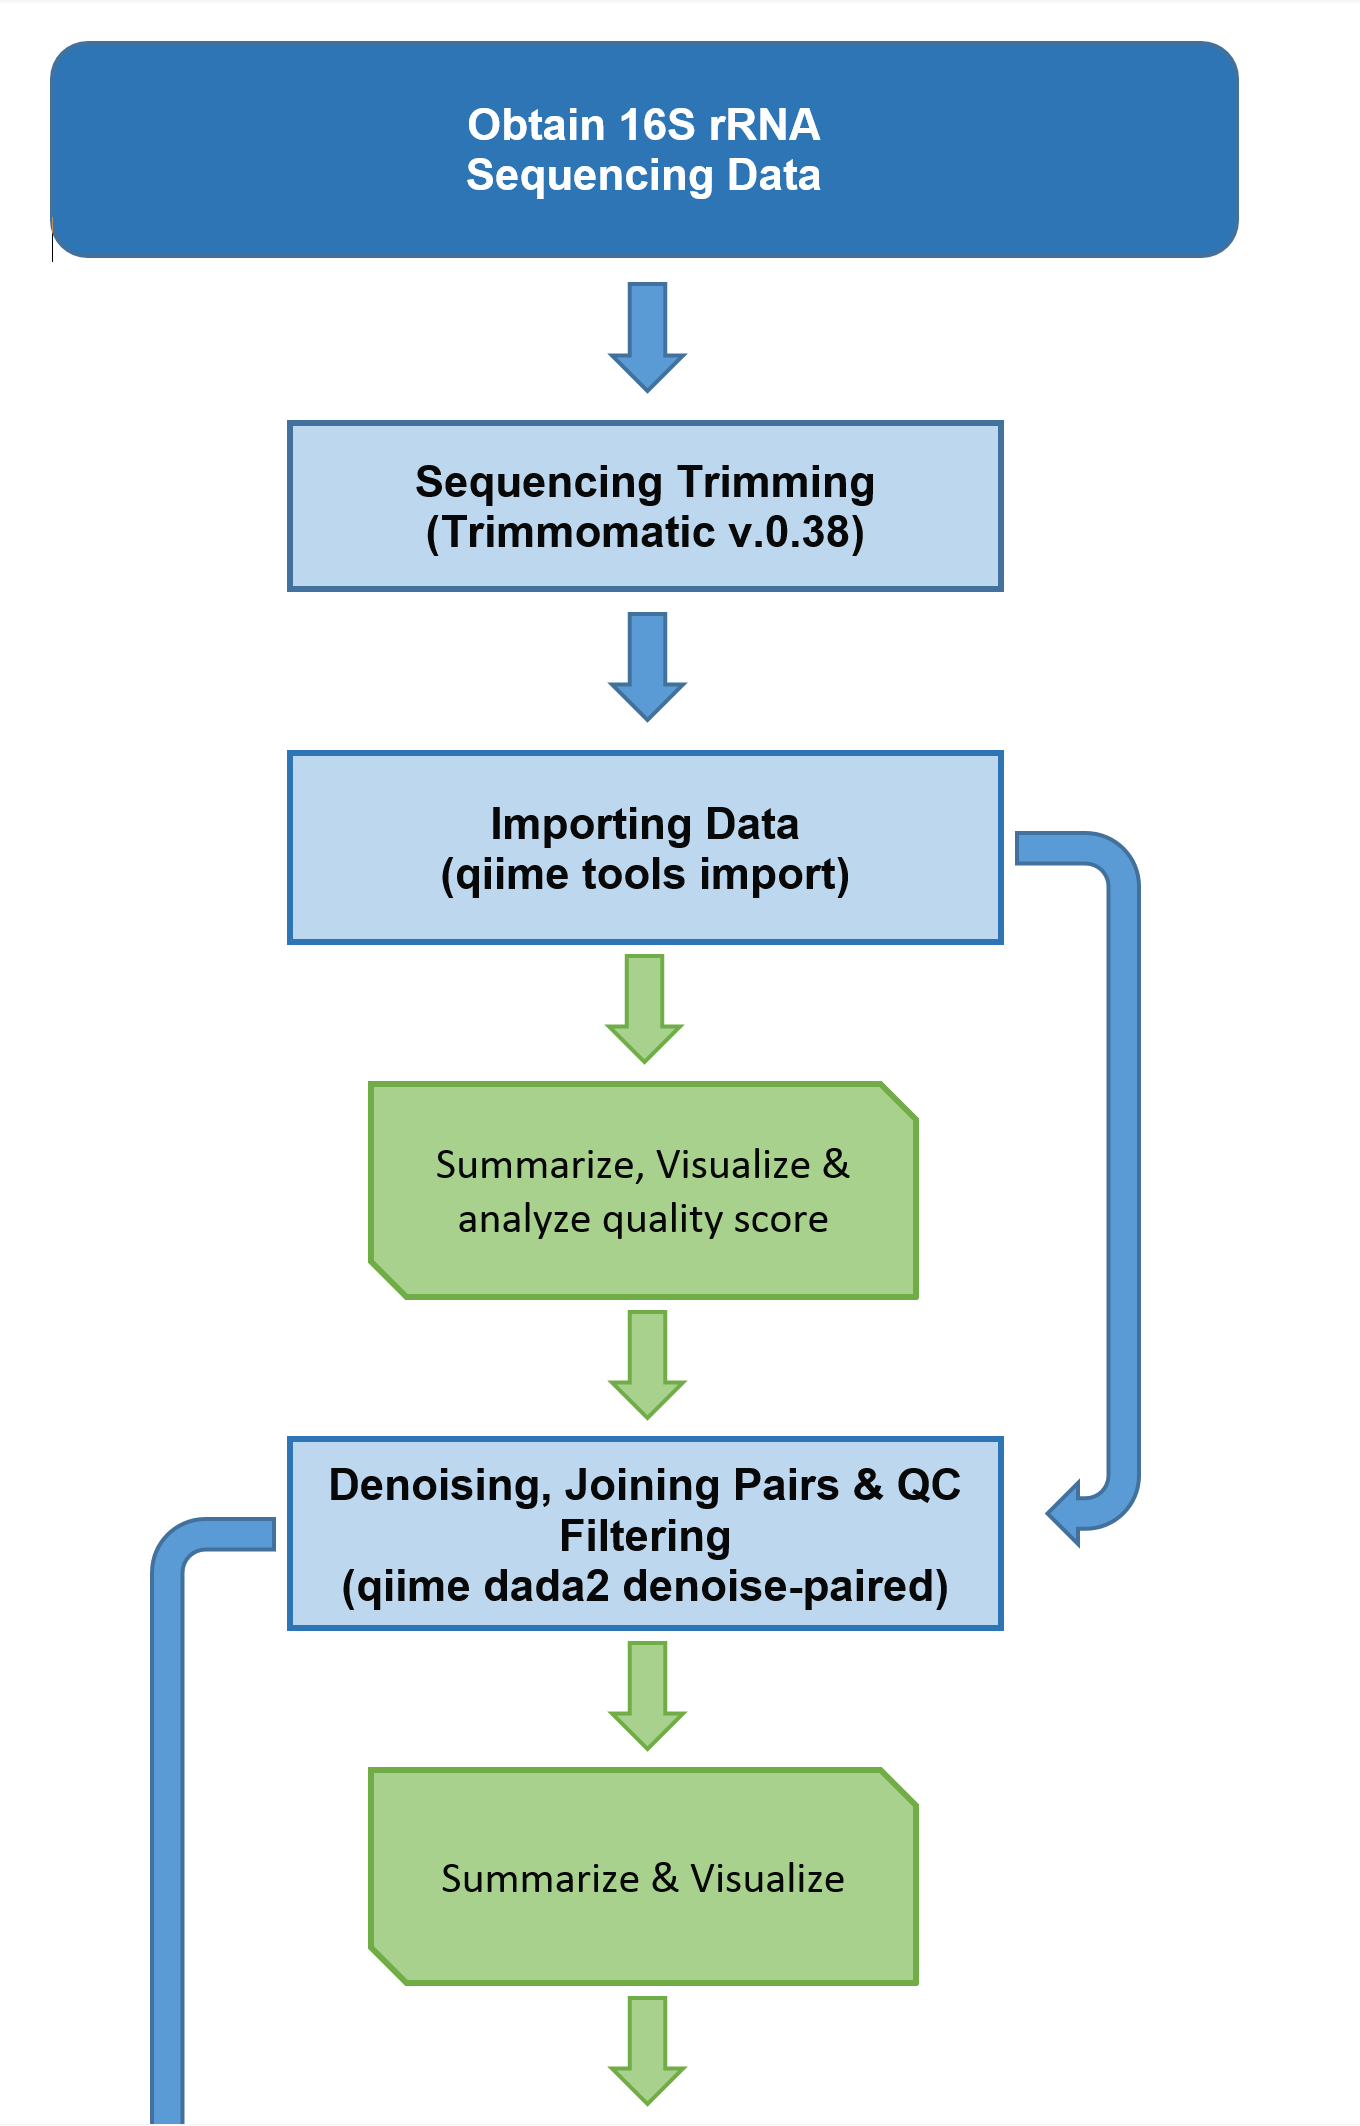
\includegraphics[scale=0.3]{figures/Workflow1.png}}
\caption{First stage of the workflow. Dataset is obtained and prepared. The blue arrow indicates major stages and the green arrow indicates summarizing and visualizing stages.}
\label{fig. 1}
\end{figure}

\begin{figure}[htbp]
\centerline{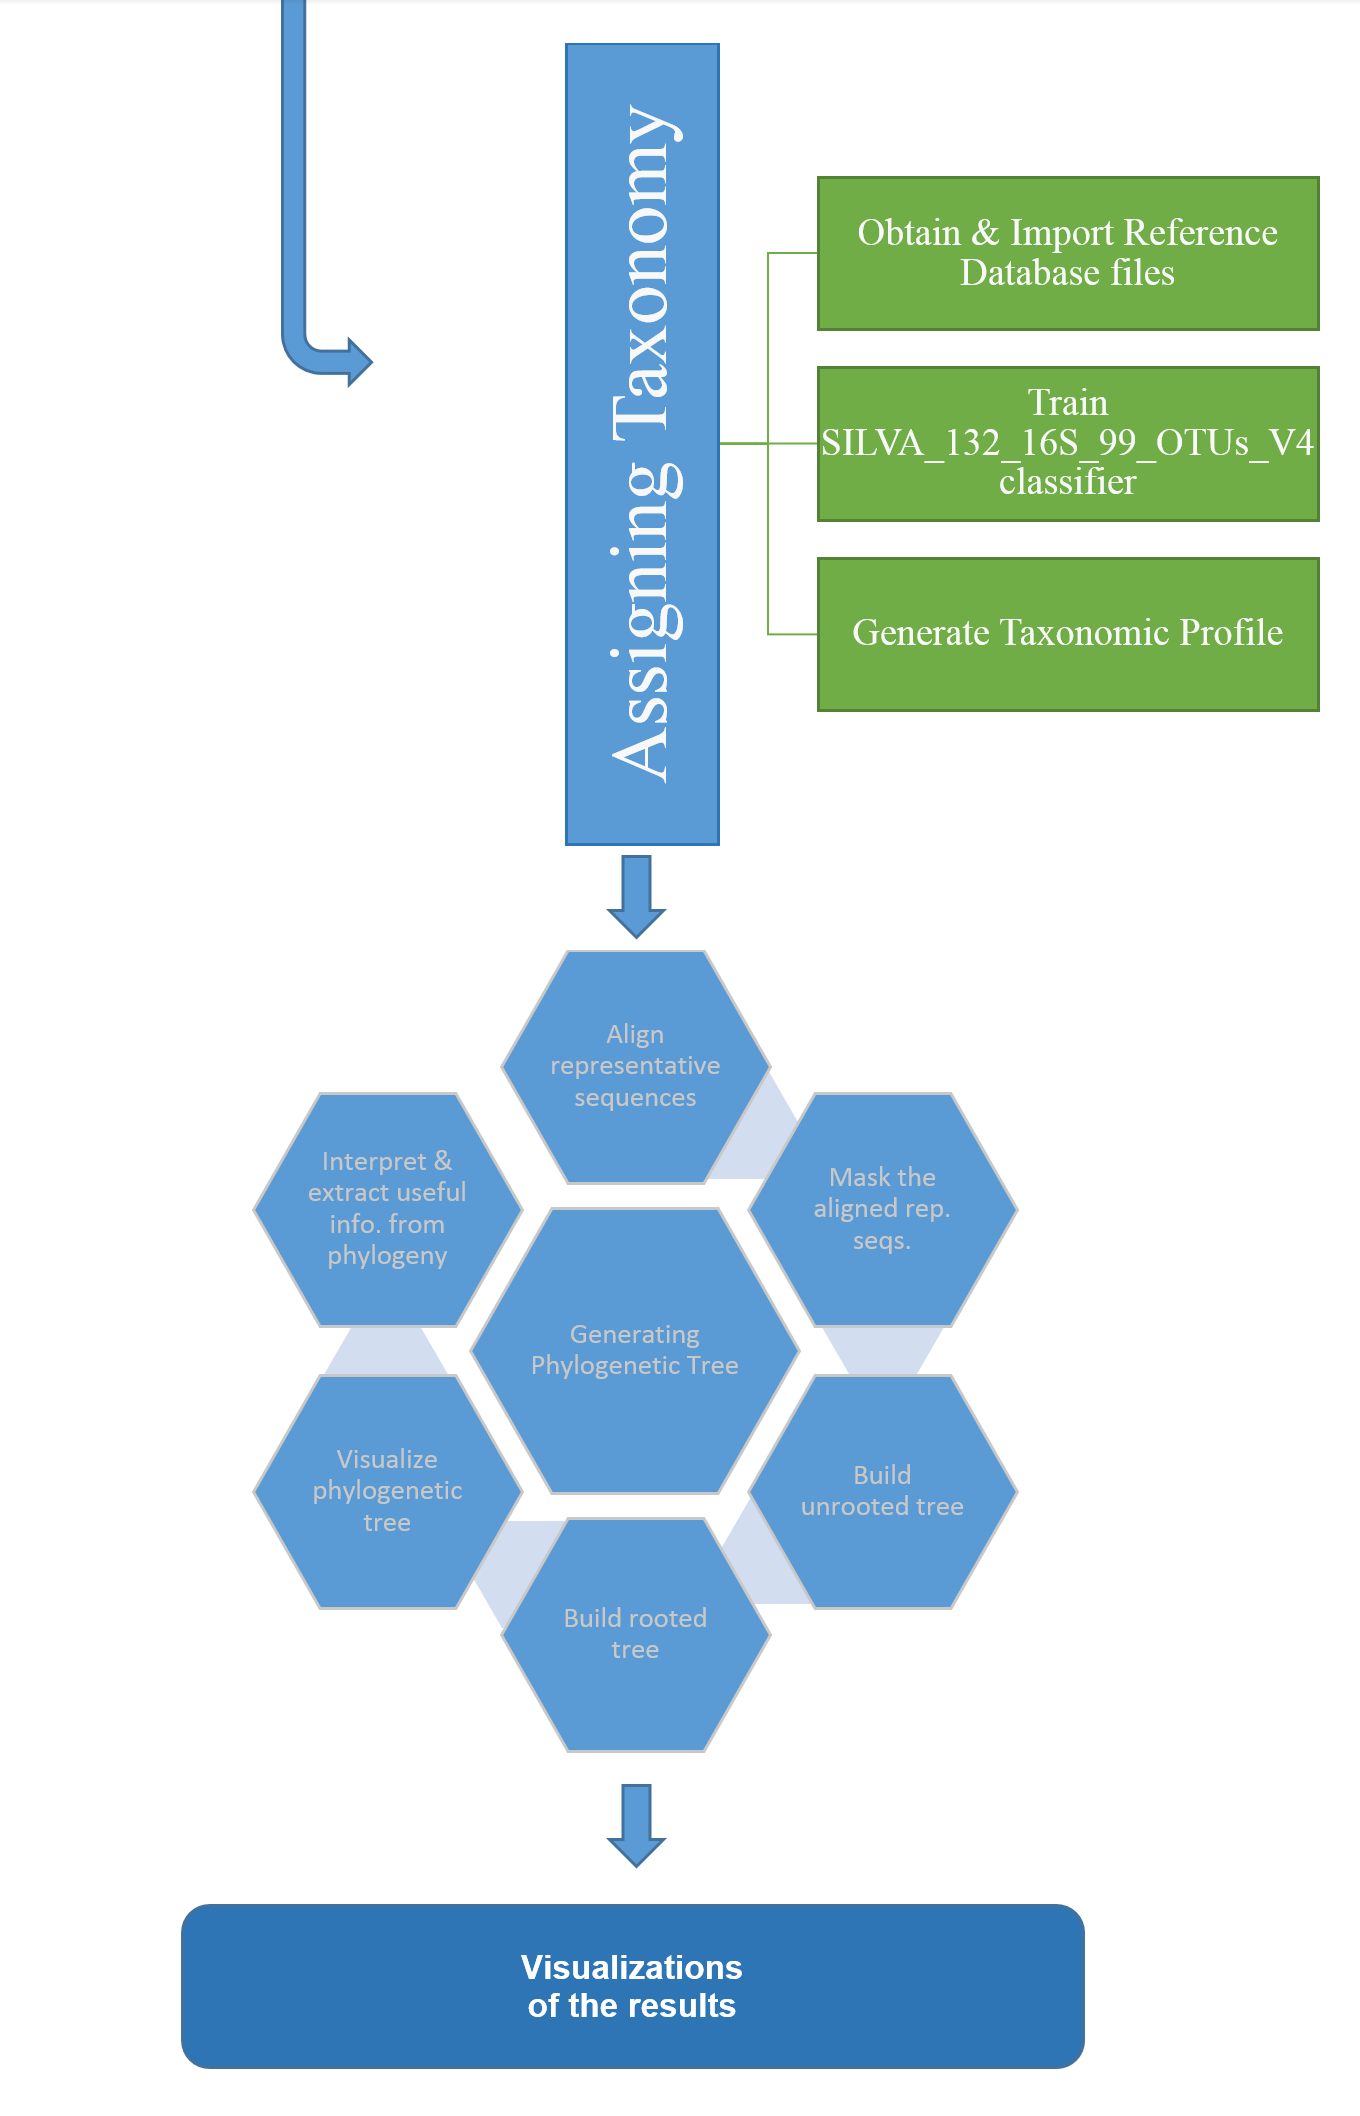
\includegraphics[scale=0.35]{figures/Workflow2.png}}
\caption{Second half of the workflow. Taxonomy and phylogeny is determined.}
\label{fig. 2}
\end{figure}

\begin{figure}[htbp]
\centerline{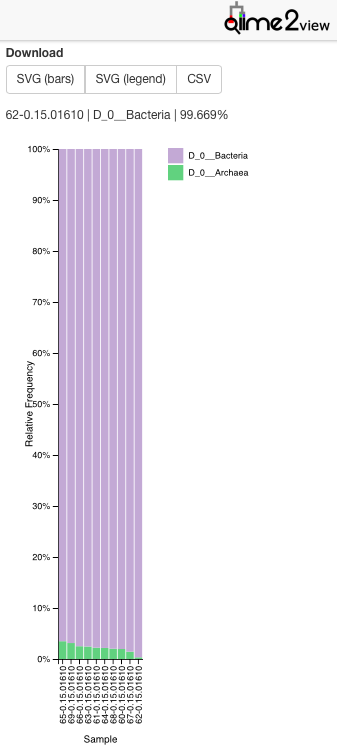
\includegraphics[scale=0.45]{figures/domain-bacteria-archaea-bp.png}}
\caption{Bar plot of ruminal microbiota composition for each sample at domain level. The purple indicates the relative frequency of \textit{bacteria} and the green indicates the relative frequency of \textit{archaea}. It is evident that more types of \textit{bacteria} are present than \textit{archaea}.}
\label{fig. 3}
\end{figure}

\begin{figure}[htbp]
\centerline{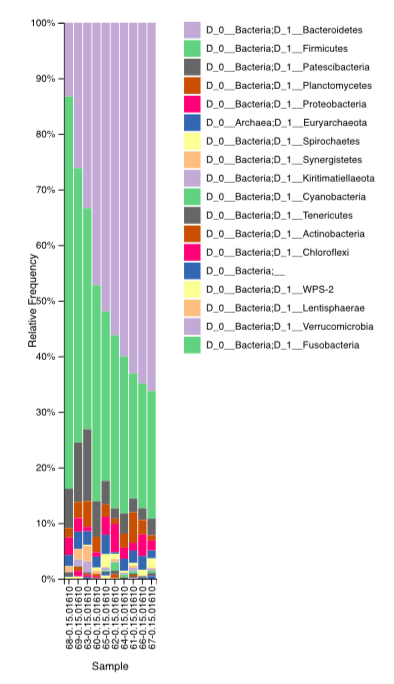
\includegraphics[scale=0.45]{figures/kingdom-bp.png}}
\caption{Bar plot of ruminal microbiota composition for each sample at kingdom level. The most common kingdoms identified in the samples were \textit{Bacteroidetes} (purple) and \textit{Firmicutes} (green).}
\label{fig. 4}
\end{figure}

\begin{figure}[htbp]
\centerline{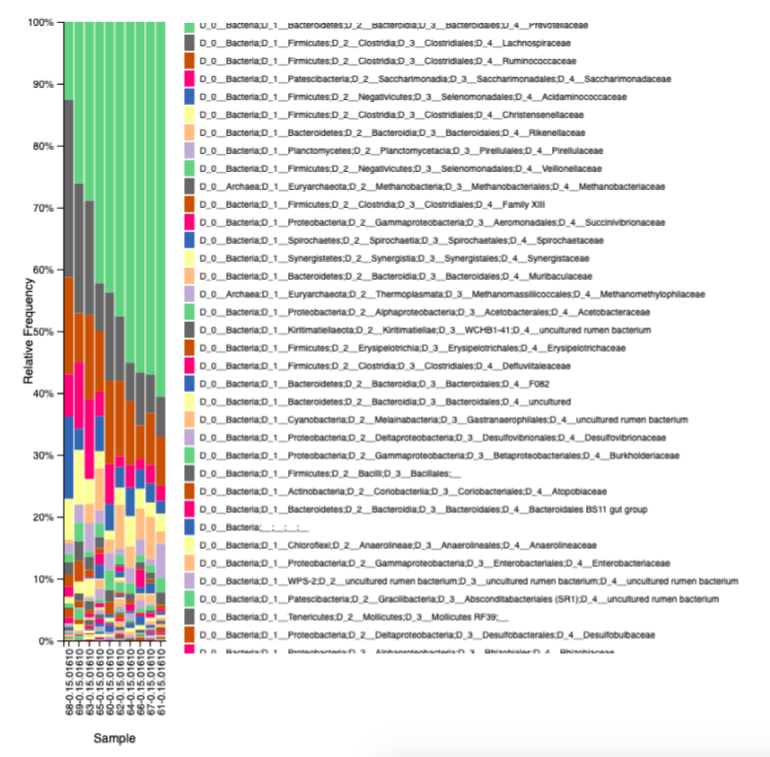
\includegraphics[scale=0.3]{figures/order-bp-w-legend.png}}
\caption{Bar plot of ruminal microbiota composition for each sample at \textit{order} level. The order was the lowest taxonomy level at which the majority of samples could be identified.}
\label{fig. 5}
\end{figure}

\begin{figure}[htbp]
\centerline{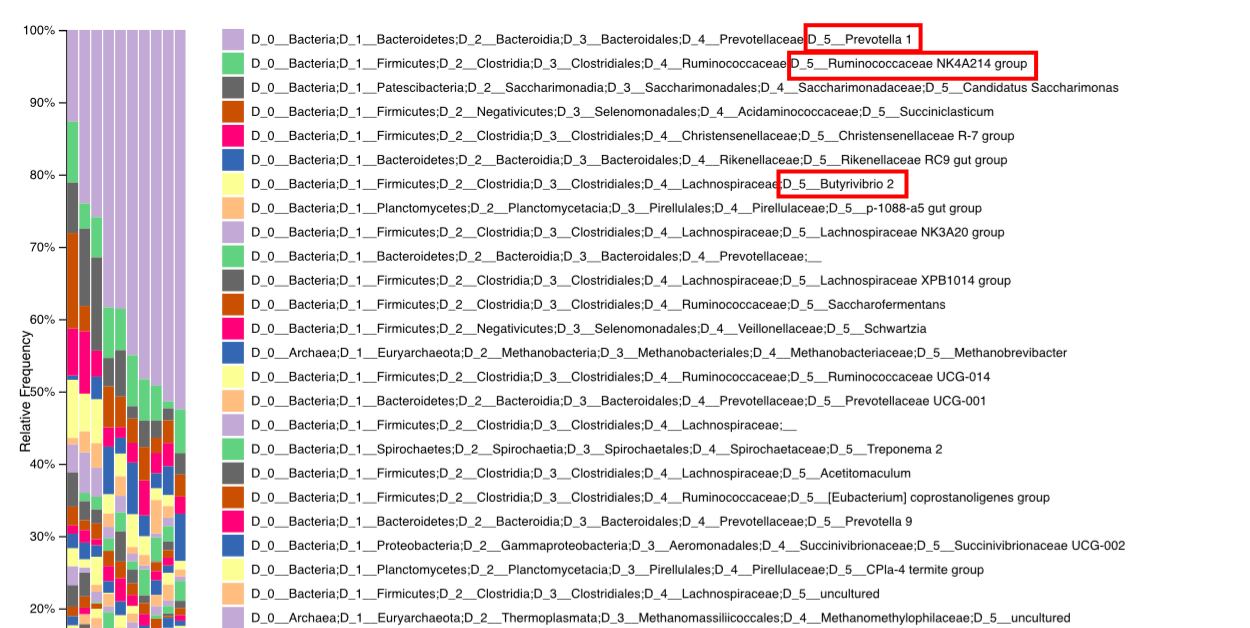
\includegraphics[scale=0.2]{figures/common-bacteria-rumen.png}}
\caption{Bar plot of ruminal microbiota composition for each sample at \textit{genus} level. \textit{Prevotella}, \textit{Butyrivibrio}, and \textit{Ruminococcus}, bacteria most commonly found in the rumen as indicated by Matthews et al., are also found in this study (marked in red boxes).}
\label{fig. 6}
\end{figure}

\begin{figure}[htbp]
\centerline{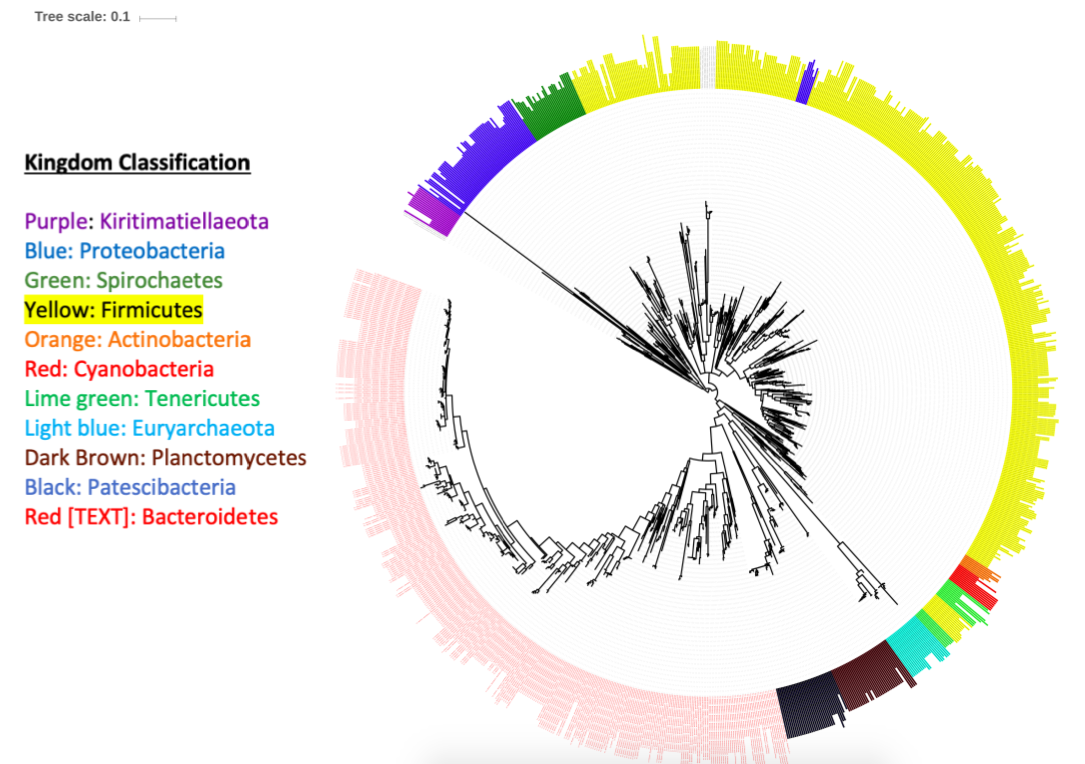
\includegraphics[scale=0.2]{figures/phylogenetic-tree-final.png}}
\caption{Phylogenetic tree with colour annotation based on kingdom-level classification.}
\label{fig. 7}
\end{figure}

\begin{figure}[htbp]
\centerline{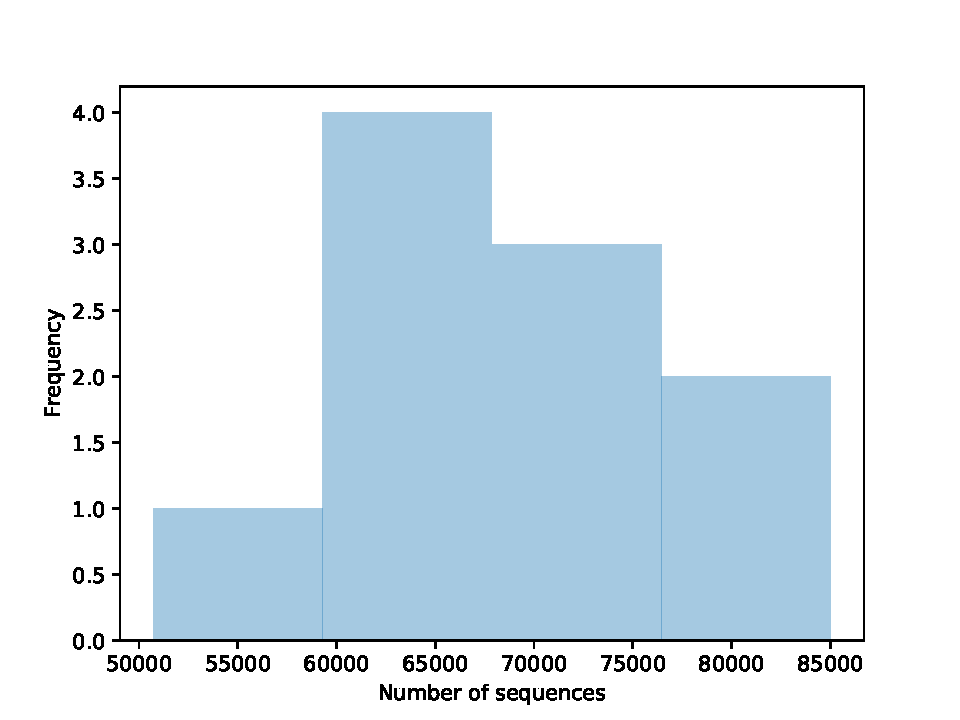
\includegraphics[scale=0.6]{figures/demultiplex-summary.pdf}}
\caption{Sequence count summary.}
\label{fig. 8}
\end{figure}

\begin{figure}[htbp]
\centerline{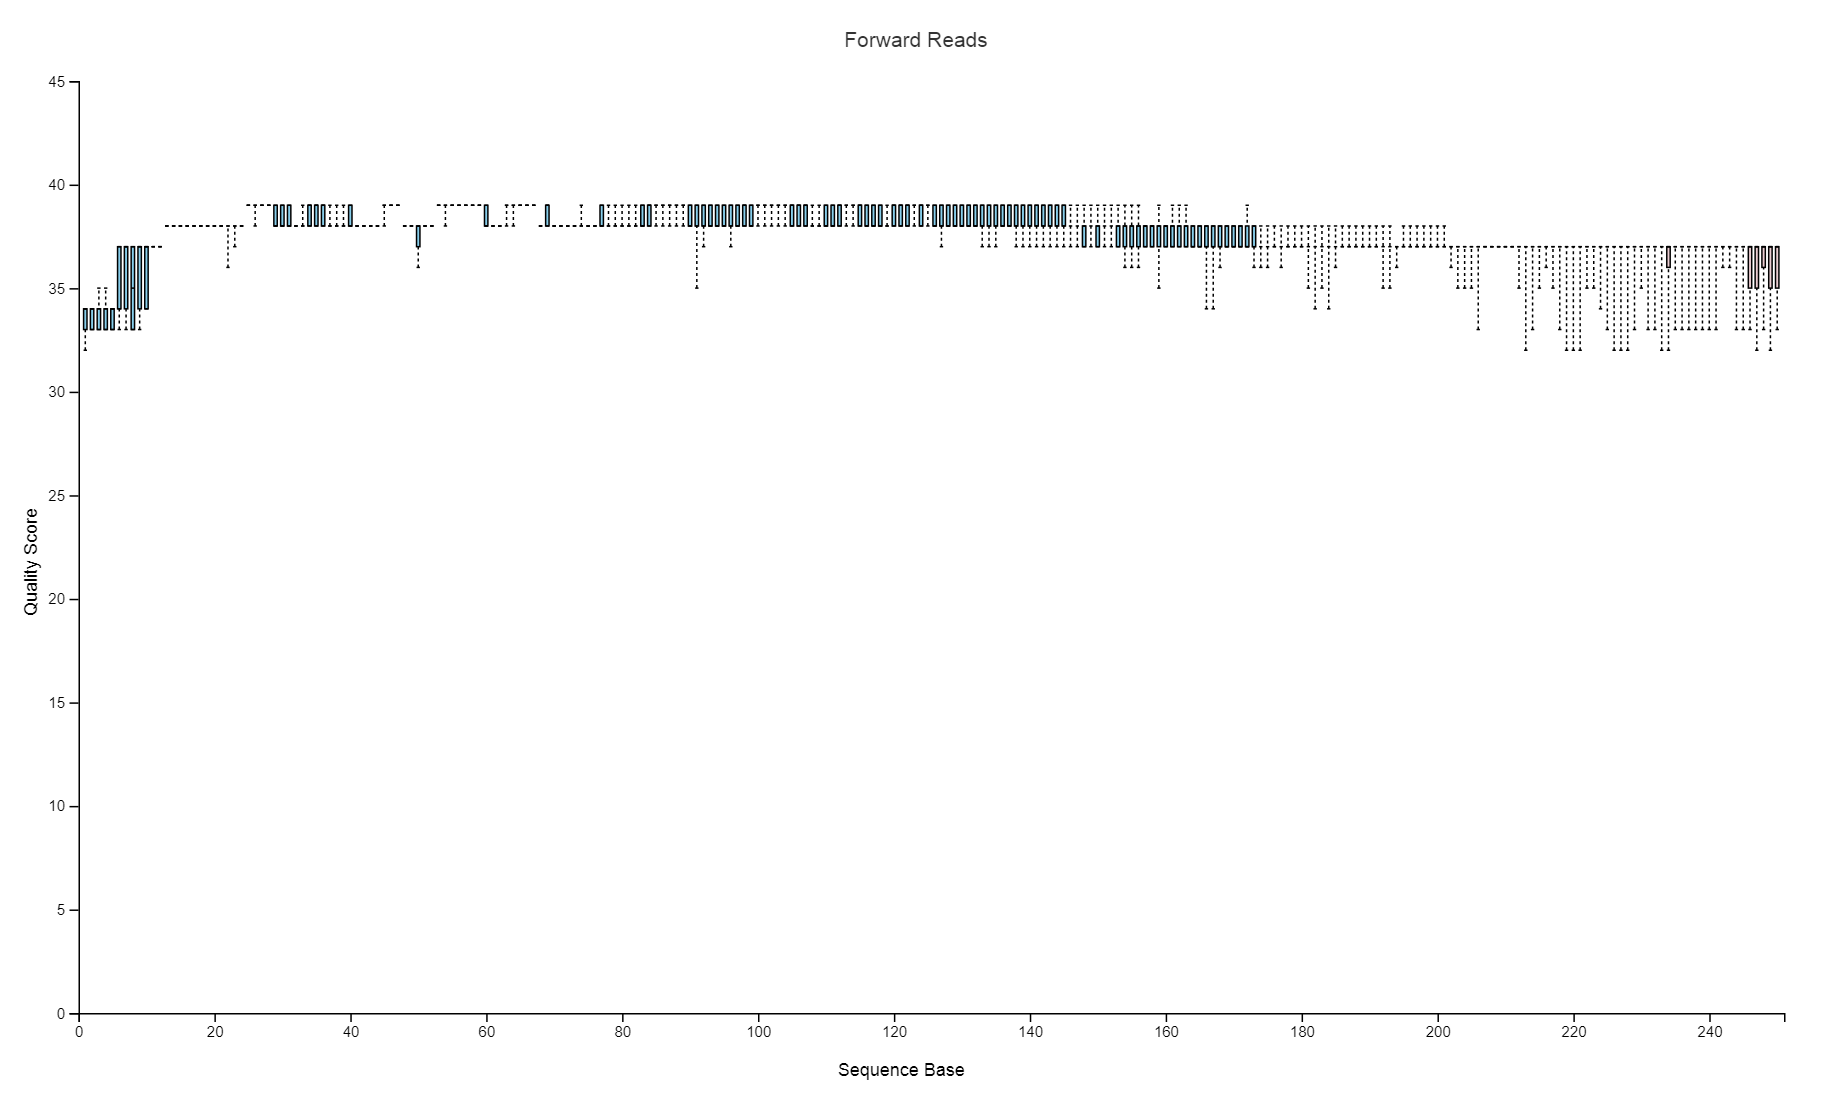
\includegraphics[scale=0.25]{figures/forward_read.png}}
\caption{Summary of length and quality score of forward reads.}
\label{fig. 9}
\end{figure}

\begin{figure}[htbp]
\centerline{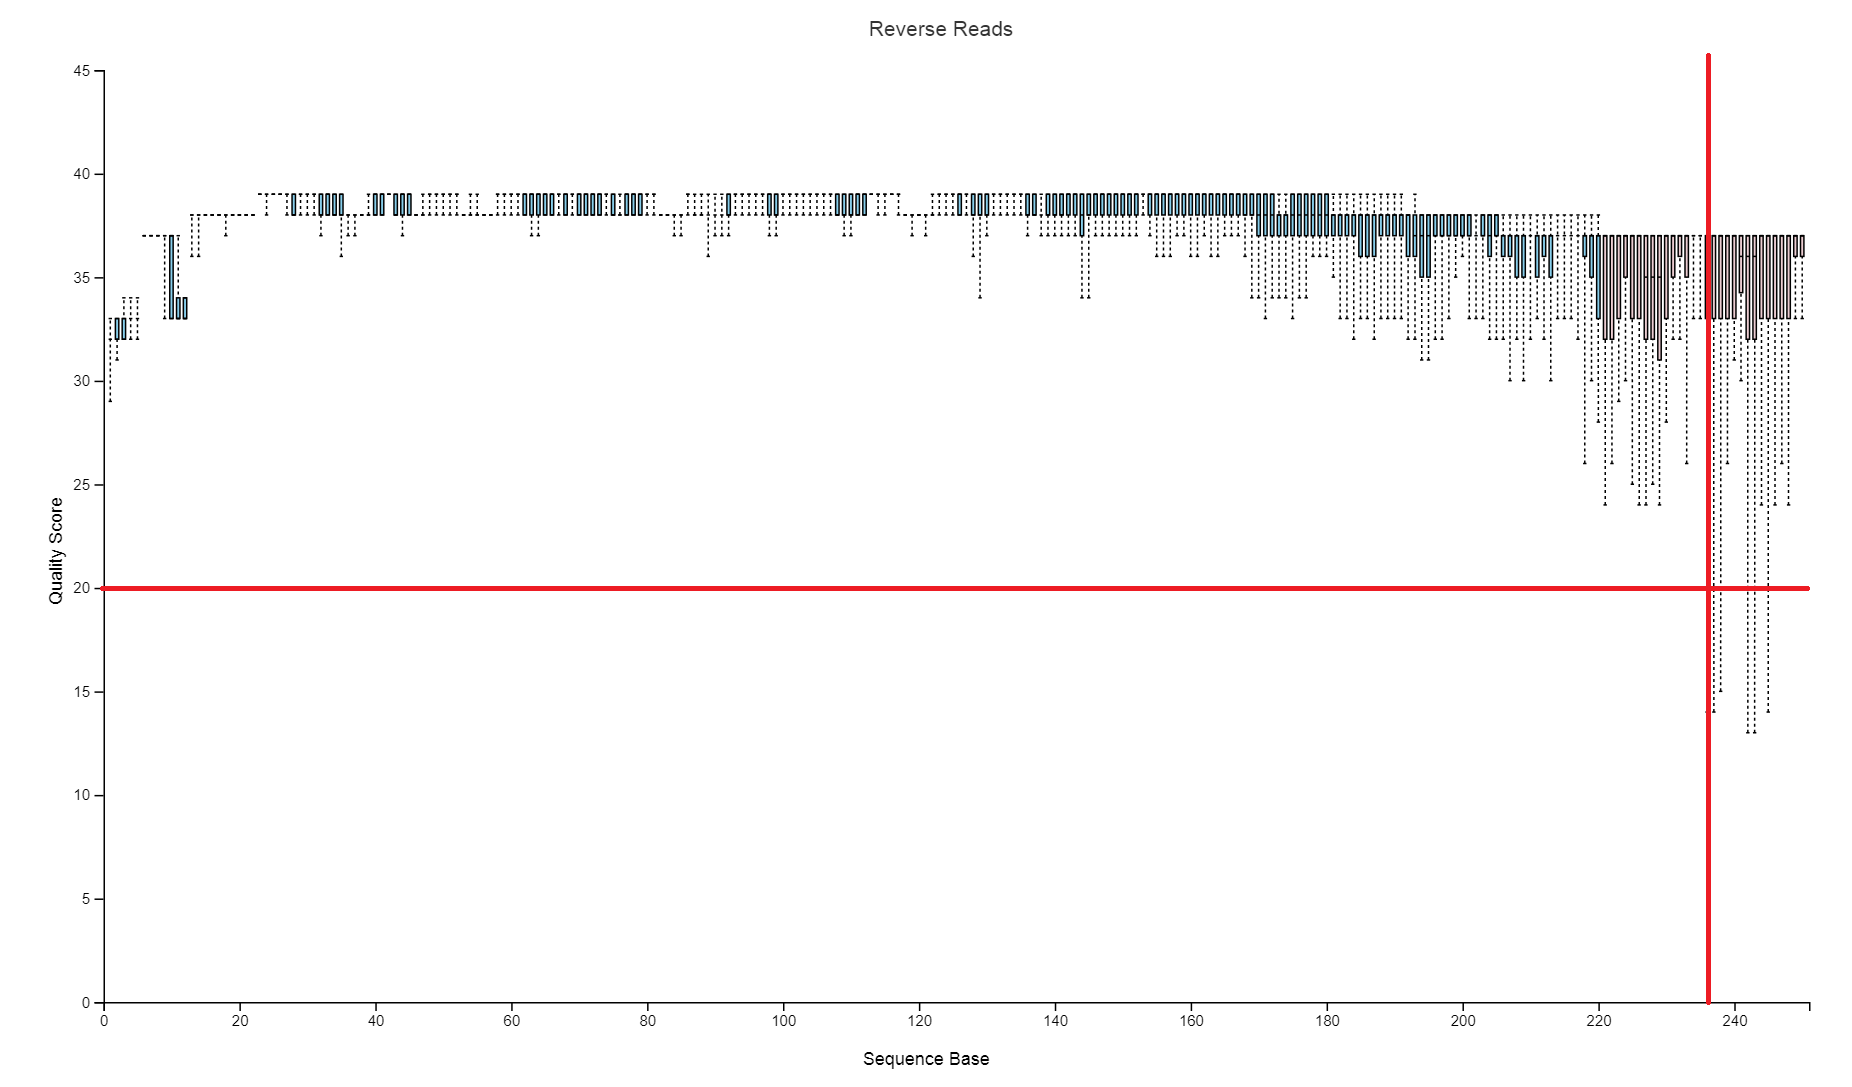
\includegraphics[scale=0.25]{figures/reverse_read.png}}
\caption{Summary of length and quality score of reverse reads. The red horizontal line marks the quality score of interest, 20. The red vertical line pinpoints the position of reads where the quality score drops below 20.}
\label{fig. 10}
\end{figure}

\pagebreak

\bibliographystyle{agsm}
\bibliography{references}
\end{document}